\documentclass[12pt,a4paper]{report}
\usepackage[left=2cm,right=2cm,top=2cm,bottom=2cm]{geometry}
\usepackage[onehalfspacing]{setspace}

\usepackage[T1]{fontenc}
\usepackage[utf8]{inputenc}
\usepackage[ngerman]{babel}
\usepackage{pifont}

\usepackage{graphicx}
\usepackage[export]{adjustbox}
\usepackage[hidelinks]{hyperref}
\usepackage{wrapfig}
\usepackage{mathtools}
\usepackage{listings}
\usepackage{url}
\usepackage{tabto}
\usepackage{tikz}
\usetikzlibrary{matrix,chains,positioning,decorations.pathreplacing,arrows,calc}
\usepackage{pgfplots}
\usepackage{amsmath}
\usepackage{subfig}

\graphicspath{{C:/Jetbrains/PyCharm/WerbeSkip/thoughts/arbeit/}}

\begin{document}

\begin{titlepage}
	\centering
	{\Large Gymnasium Bäumlihof, 5Bb \par}
	\vspace{1cm}
	{\LARGE\scshape Maturaarbeit\par}
	\vspace{1.5cm}
	{\huge\bfseries Kann der Computer Werbung erkennen?\par}
	\vspace{0.6cm}
    {\Large Bilderkennung mit einem Neuronalen Netzwerk\par}
	\vspace{2cm}
	{\Large\itshape Georg Schwan\par}
	\vfill
	Betreuungsperson\par
	{\itshape Test1\par}
	Korreferent\par
	{\itshape Test2}
	\vfill
	{\large \today\par}
\end{titlepage}

\tableofcontents

\newpage

\chapter{Einleitung}\label{ch:einleitung}

\section{Motivation}
\label{sec:motivation}
Vor ein paar Jahren haben wir Fernsehen geschaut und immer wenn Werbung kam haben wir den Sender gewechselt,
bis die Werbung vorbei war und das normale Programm weiter lief.
Das Problem war nur, dass wir nie wussten wann die Werbung vorbei war.
Meinem Bruder ist aufgefallen, dass bei Werbung nie das Logo vom Sender eingespielt wird.
Daraufhin hat er probiert ein Algorithmus zu schreiben, der das Logo von einem Sender erkennen kann.
Er versuchte das Logo mithilfe von Bedingungen und Schleifen auszudrücken, aber vergebens.

Als ich auf der Suche nach einer Idee für eine Maturaarbeit war erinnerte ich mich wieder an das Problem und an einen neuen Lösungsansatz,
nämlich Neuronale Netzwerke, welche Heute überall verwendet werden und extrem Mächtig sind.
Die Idee war aber nicht nur ein Logo zu erkennen sondern auch genau verstehen wie ein Neuronales Netzwerk funktioniert
und deshalb habe ich mein eigenes Neuronale Netzwerk programmiert.
\section{Aufbau der Arbeit}
\label{sec:aufbauDerArbeit}

\chapter{Problemstellung}
Das Ziel dieser Arbeit ist einen Algorithmus zu programmieren der Bilder als Werbung erkennen kann.
Dafür wrd ein Neuronales Netzwerk benutzt, das sich auf die Bilderkennung beschränkt.
\section{Werbung}
Wie schon gesagt wird bei Werbung das Senderlogo nicht eingeblendet und deswegen kann das Problem
vereinfacht werden auf die Frage ob das Senderlogo eingeblendet ist oder nicht (siehe Abbildung~\ref{fig:logo1}).

\begin{figure}[h]%
    \centering
    \subfloat[Werbung]{{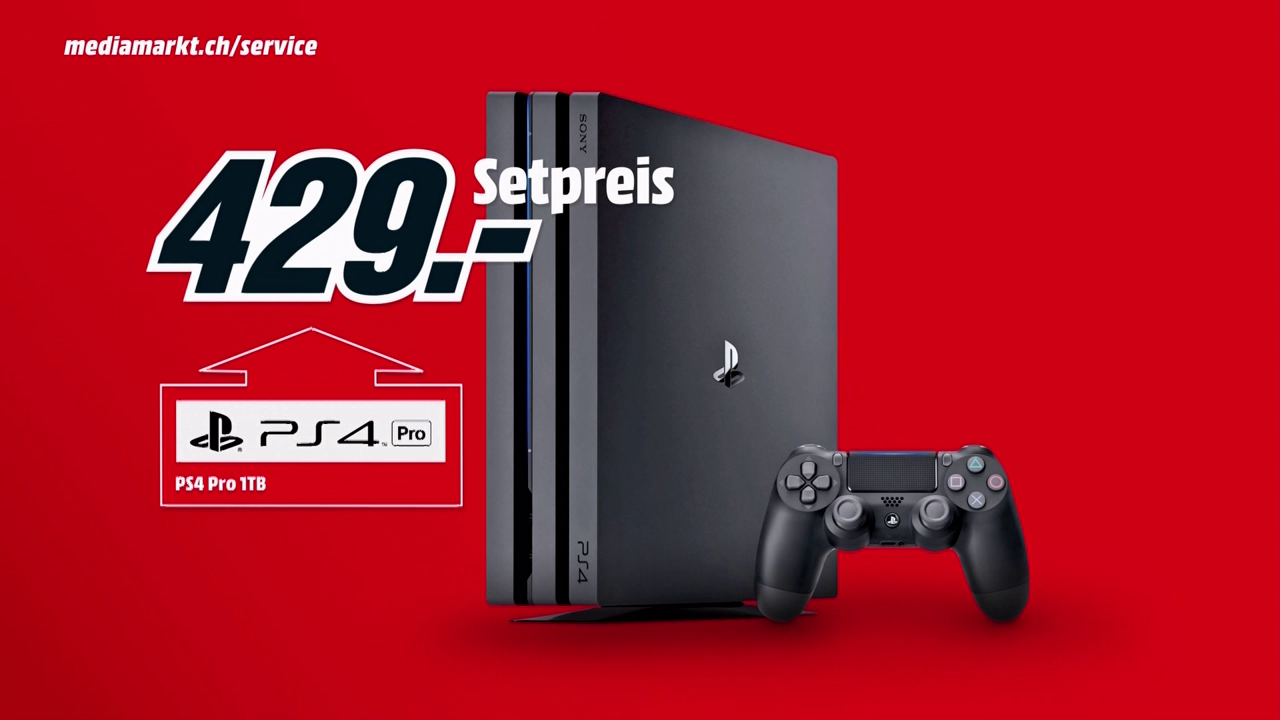
\includegraphics[width=7cm]{assets/images/prosieben_kein_logo.png} }}%
    \qquad
    \subfloat[Keine Werbung]{{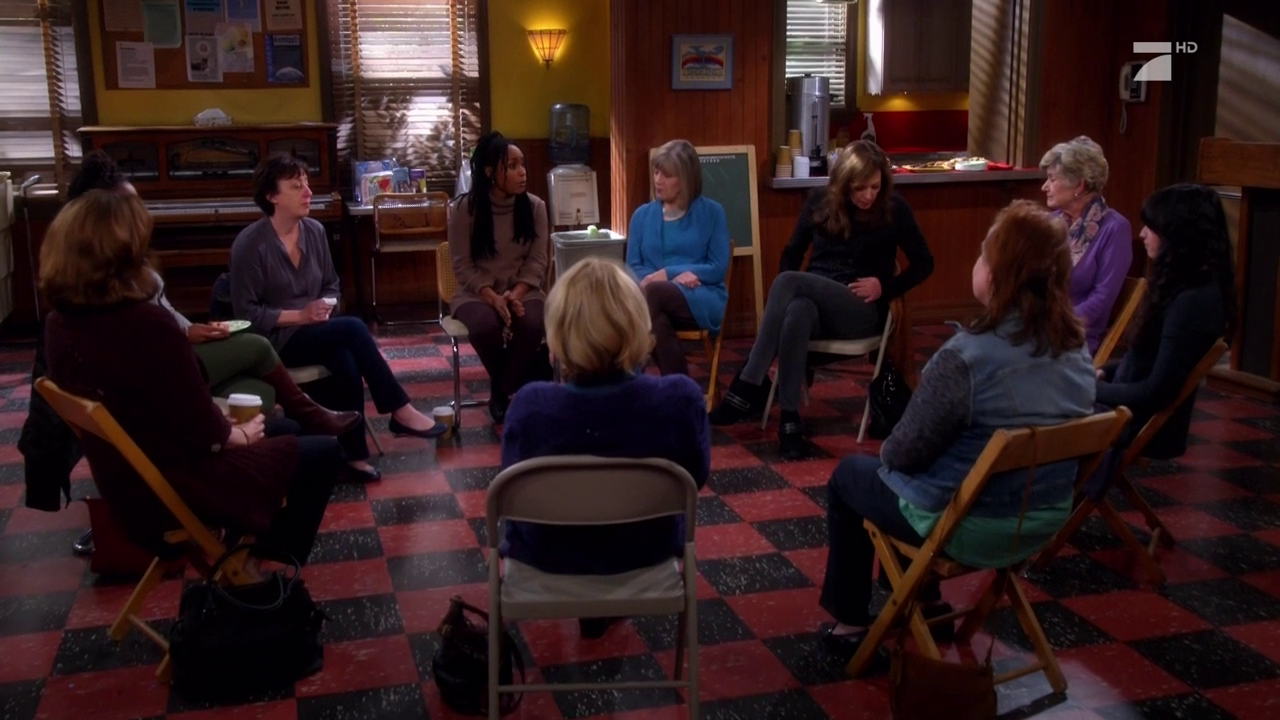
\includegraphics[width=7cm]{assets/images/prosieben_logo.png} }}%
    \caption{Kein Senderlogo bei Werbung}%
    \label{fig:logo1}%
\end{figure}

\section{Neuronales Netzwerk}
Neuronale Netzwerke sind ein sehr umfangreiches Thema und deswegen begrenze ich mich auf Netzwerke die für die Bilderkennung entscheidend sind.
Darunter sind klassische feedforward und convolution Netzwerke.
Auf recurrent neuronale Netzwerke\footnote{Ein Neuronales Netzwerk, das geeignet für Sequenzen ist} wird nicht näher eingegangen.


\chapter{Neuronales Netzwerk}
\label{ch:neuronalesNetzwerk}
Dieses ganze Kapitel bezieht sich auf das Buch von Michael A. Nielsen\cite{neuralbook}, ausser es ist anders deklariert.
\section{Konzept}\label{sec:konzept}
Wenn man ein normales Programm schreiben will muss man das Problem in viele kleinere aufteilen, bis der Computer fähig ist,
es zu lösen.
In einem Neuronale Netzwerk wird dem Computer nicht gesagt wie es das Problem lösen kann, sondern ein Neuronales Netzwerk
versteht das Problem, indem wir es Beispieldaten geben und es daran lernen kann, bis es seine eigene Lösung gefunden hat.
Zum Beispiel, wir wollen einem Netzwerk beibringen ob in einem Bild ein Auto vorkommt,
dazu geben wir dem Neuronale Netzwerk viele Bilder, mit und ohne Auto.
Mit jedem Bild, dass das Neuronale Netzwerk bekommt, lernt es besser wie ein Auto ausschaut.

Das Konzept eines Neuronales Netzwerk ist nicht etwas neuses.
Im Jahre 1957 hat Frank Rosenblatt ein erste Idee eines Neuronales Netzwerk vorgestellt, aber erst in den letzten
Jahren ist der grosse Hype ausgebrochen, dies liegt daran, dass man erst jetzt die nötigen Daten
und Rechenleistung zu verfügung hat.

\section{Neuron}\label{sec:neuron}
User Gehirn kann Entscheidungen treffe, da wir billionen von Neuronen haben, die miteinander verbunden sind und sich
verständigen können.
Aber ein Neuron an sich ist praktisch nutzlos, aber in grosser Anzahl können sie komplexeste Probleme lösen.

Nach dem gleichen Prinzip funktioniert ein Neuronales Netzwerk
Es besteht aus vielen Neuronen (daher der Name) die miteinander verbunden sind.


\begin{figure}[h]
    \centering
\begin{tikzpicture}[
init/.style={
  draw,
  circle,
  inner sep=2pt,
  font=\Huge,
  join = by -latex
},
squa/.style={
  draw,
  inner sep=2pt,
  font=\Large,
  join = by -latex
},
start chain=2,node distance=13mm
]
\node[on chain=2]
  (x2) {$x_2$};
\node[on chain=2,join=by o-latex]
  {$w_2$};
\node[on chain=2,init] (sigma)
  {$\displaystyle\Sigma$};
\node[on chain=2,squa,label=above:{\parbox{2cm}{\centering Activate \\ function}},join=by -latex, minimum size=0.9cm]
  {$f$};
\node[on chain=2,label=above:Ausgabe,join=by -latex]
  {$y$};
\begin{scope}[start chain=1]
\node[on chain=1] at (0,1.5cm)
  (x1) {$x_1$};
\node[on chain=1,join=by o-latex]
  (w1) {$w_1$};
\end{scope}
\begin{scope}[start chain=3]
\node[on chain=3] at (0,-1.5cm)
  (x3) {$x_3$};
\node[on chain=3,label=below:Gewichte,join=by o-latex]
  (w3) {$w_3$};
\end{scope}
\node[label=above:\parbox{2cm}{\centering Bias \\ $b$}] at (sigma|-w1) (b) {};

\draw[-latex] (w1) -- (sigma);
\draw[-latex] (w3) -- (sigma);
\draw[o-latex] (b) -- (sigma);

\draw[decorate,decoration={brace,mirror}] (x1.north west) -- node[left=10pt] {Eingabe} (x3.south west);
\end{tikzpicture}
    \caption{Einzelner Neuron in einem Neuronalen Netzwerks}
    \label{fig:neuron1}
\end{figure}

Ein Neuron in einem Neuronales Netzwerk wird als Mathematische funktion definiert wie Abbildung~\ref{fig:neuron1}
verdeutlicht.
Ein Neuron hat $n$ verschiedene Eingaben, die als $x_j$ bezeichnet werden und mit einem spezifischen Gewicht $w_j$ multipliziert werden.
Die Ausgabe erfolgt indem man alle gewichteten Eingaben, mit einem Bias $b$, addiert und durch eine so genannte
Aktivierungsfunktion $f$ durchlaufen läst.
Als Gleichung:
\[y =f\left(\sum_{j=1}^{n} x_j w_j + b\right)\]
Die Gewichte $w_j$ und der Bias $b$ des Neurons sind die Parameter, die angepasst werden und somit das Neuron lernfähig machen.

Eine Aktivierungsfunktion ist nötig, da ohne eine wäre ein Neuronales Netzwerk eine komplett lineare funktion, welches
nur lineare Probleme lösen könnte.\cite{activations}
Die meisten Probleme sind viel komplexer als das man sie linear darstellen könnte und deswegen ist eine Aktivierungsfunktion von nötig.
Es wird näher auf die Aktivierungsfunktion eingegangen im Abschnitt~\ref{sec:aktivierungsfunktionen}

\section{Architektur}
Wie auch im biologischen Gehirn ist ein Neuron allein nutzlos.
Erst wenn man die Neuronen miteinander verbindet kann es komplexe Zusammenhänge modellieren.
\begin{figure}[h]
    \centering
\begin{tikzpicture}[
plain/.style={
  draw=none,
  fill=none,
  },
net/.style={
  matrix of nodes,
  nodes={
    draw,
    circle,
    inner sep=10pt
    },
  nodes in empty cells,
  column sep=2cm,
  row sep=-9pt
  },
>=latex
]
\matrix[net] (mat)
{
|[plain]| \parbox{1.3cm}{\centering} & |[plain]| \parbox{1.3cm}{\centering} & |[plain]| \parbox{1.3cm}{\centering} \\
& |[plain]| \\
|[plain]| & \\
& |[plain]| \\
  |[plain]| & |[plain]| \\
& & \\
  |[plain]| & |[plain]| \\
& |[plain]| \\
  |[plain]| & \\
& |[plain]| \\    };
\foreach \ai [count=\mi ]in {2,4,...,10}
  \draw[<-] (mat-\ai-1) -- node[above] {Eingabe $x_\mi$} +(-2.8cm,0);
\foreach \ai in {2,4,...,10}
{\foreach \aii in {3,6,9}
  \draw[->] (mat-\ai-1) -- (mat-\aii-2);
}
\foreach \ai in {3,6,9}
  \draw[->] (mat-\ai-2) -- (mat-6-3);
\draw[->] (mat-6-3) -- node[above] {Ausgabe} +(2.5cm,0);
\end{tikzpicture}
    \caption{Mögliche architektur eines Neuronalen Netzwerk}
    \label{fig:network1}
\end{figure}

Eine mögliche Architektur kann wie in  Abbildung~\ref{fig:network1} ausschauen.
Ein Netzwerk wird generell immer in verschiedene Schichten unterteilt.
Die linke Schicht wird als eingabe Schicht bezeichnet und die Neuronen in dieser Schicht werden eingabe Neuronen genannt.
Analog da zu wird die rechte Schicht ausgabe Schicht genannt, die die ausgabe Neuronen beinhaltet.
Die mittleren Schichten, die von der Anzahl variieren können, werden versteckte Schichten genannt.
Die Anzahl der Neuronen in jeder Schicht kann auch variieren.
Abbildung~\ref{fig:network2} zeigt eine andere mögliche Architektur für ein Netzwerk, welches 2 versteckte
Schichten hat.
\begin{figure}[h]
    \centering
\begin{tikzpicture}[
plain/.style={
  draw=none,
  fill=none,
  },
net/.style={
  matrix of nodes,
  nodes={
    draw,
    circle,
    inner sep=10pt
    },
  nodes in empty cells,
  column sep=2cm,
  row sep=-9pt
  },
>=latex
]
\matrix[net] (mat)
{
|[plain]|  & |[plain]|  & |[plain]|  & |[plain]| \\
& |[plain]|& |[plain]|& |[plain]| \\
|[plain]| && |[plain]|& |[plain]| \\
& |[plain]|&& |[plain]|& |[plain]| \\
  |[plain]| && |[plain]|&& |[plain]| \\
& |[plain]| & \\
  |[plain]| && |[plain]|&& |[plain]| \\
& |[plain]| && |[plain]|& |[plain]|  \\
  |[plain]| & & |[plain]|& |[plain]|  \\
& |[plain]|& |[plain]|& |[plain]| \\     };
\foreach \ai in {2,4,...,10}
{\foreach \aii in {3,5, 7,9}
  \draw[->] (mat-\ai-1) -- (mat-\aii-2);
}
\foreach \ai in {3,5,7,9}
{\foreach \aii in {4,6,8}
  \draw[->] (mat-\ai-2) -- (mat-\aii-3);
}
\foreach \ai in {4,6,8}
{\foreach \aii in {5, 7}
  \draw[->] (mat-\ai-3) -- (mat-\aii-4);
}
\draw[decorate,decoration={brace}] (mat-1-1.west) -- node[above=5pt] {\parbox{3cm}{\centering Eingabe\\Schicht}} (mat-1-1.east);
\draw[decorate,decoration={brace}] (mat-1-2.west) -- node[above=5pt] {\parbox{3cm}{\centering Versteckte\\Schichten}} (mat-1-3.east);
\draw[decorate,decoration={brace}] (mat-1-4.west) -- node[above=5pt] {\parbox{3cm}{\centering Ausgabe\\Schicht}} (mat-1-4.east);
\draw[decorate,decoration={brace,mirror}] ($(mat-1-1.west)+(-0.1cm,-0.2cm)$) -- node[left=5pt] {\parbox{2cm}{\centering Eingabe\\Neuronen}} ($(mat-10-1.west) + (-0.1cm,-16pt)$);
\draw[decorate,decoration={brace}] ($(mat-5-4.east)+(+0.1cm,+16pt)$) -- node[right=5pt] {\parbox{2cm}{\centering Ausgabe\\Neuronen}} ($(mat-7-4.east) + (+0.1cm,-16pt)$);
\end{tikzpicture}
    \caption{Neuronales Netzwerk mit 2 versteckten Schichten}
    \label{fig:network2}
\end{figure}
Jeder Neuron von der vorigen Schicht ist mit jedem Neuron der nachfolgenden Schicht verbunden.
Dies ist ein klassisches feedforawrd Netzwerk.
Wichtig zu beachten ist, dass keine Schleifen vorkommen.

\subsection{Beschriftung}

Um eine allgemeine Gleichung zu bestimmen, muss man zuerst die Elemente des Netzwerks benennen.
Wir bezeichnen das Gewicht $w^l_{k,j}$ für die Verbindung des $k^{ten}$ Neuron der $(l-1)^{ten}$ Schicht
zu dem $j^{ten}$ Neuron der $l^{ten}$ Schicht.
Ähnlich dazu bezeichnen wir die Ausgabe des Neurons als $a^l_j$ und der bias des Neurons als $b^l_j$ (siehe Abbildung~\ref{fig:network3}).

\begin{figure}[h]
    \centering
\begin{tikzpicture}[
plain/.style={
  draw=none,
  fill=none,
  },
net/.style={
  matrix of nodes,
  nodes={
    draw,
    circle,
    inner sep=10pt
    },
  nodes in empty cells,
  column sep=2cm,
  row sep=-9pt
  },
>=latex
]
\matrix[net] (mat)
{
|[plain]| \parbox{2cm}{\centering Schicht 1} & |[plain]| \parbox{2cm}{\centering Schicht 2} & |[plain]| \parbox{2cm}{\centering Schicht 3} \\
& |[plain]| \\
|[plain]| & \\
& |[plain]| \\
  |[plain]| & |[plain]| \\
& & \\
  |[plain]| & |[plain]| \\
& |[plain]| \\
  |[plain]| & \\
& |[plain]| \\    };
\foreach \ai in {2,4,...,10}
{\foreach \aii in {3,6,9}
  \draw[->] (mat-\ai-1) -- (mat-\aii-2) coordinate[midway](center1\ai\aii);
}
\foreach \ai in {3,6,9}
  \draw[->] (mat-\ai-2) -- (mat-6-3) coordinate[midway](center2\ai);


\node[] at (mat-8-1)
  (x3) {$b^1_4$};
\node[] at (mat-3-2)
  (x3) {$a^2_1$};

\node (h1) at (-1.5, 2.2) {$w^2_{1,2}$};

\draw[->] (h1) -- (center126);

\node (h2) at (3, 1.5) {$w^3_{3,1}$};

\draw[->] (h2) -- (center29);

\end{tikzpicture}
    \caption{Bezeichnung der Parameter}
    \label{fig:network3}
\end{figure}
Mit dieser Notation kann eine Gleichung für das Netzwerk aufgestellt werden, welche der Gleichung einem Neuron ähnelt~\ref{sec:neuron}.

\[a^l_j = f\left(\sum_{k} a^{l-1}_k w^l_{k,j} + b^l_j\right)\]

\section{Wie das Netzwerk lernt}\label{sec:lernen}
Bis jetzt ging es nur darum wie ein Neuronales Netzwerk aufgebaut ist.
In dem Abschnitt geht wie ein Neuronales Netzwerk, anhand von Daten, lernen kann
\subsection{Kostenfunktion}
Damit ein Netzwerk lernen kann muss man dem Netzwerk zuerst sagen können wie gut oder wie schlecht es gerade ist.
Dazu definieren wir eine Kostenfunktion $C$, die von allen Gewichten $w$ und allen biases $b$ abhängig ist.
Das Netzwerk wird als Funktion $y(x)$ bezeichnet.
Den Eingabewert wird als $x$ bezeichnet mit dem dazugehörige Label $l$.
Beachte, dass $x$ und $l$ Vektoren sind.
Zum Beispiel würde ein Bild, das 10x10 Pixel gross ist, einen ($10 * 10 =$)100-dimensionaler Vektor haben
und das Label, wenn es 3 ausgabe Neuronen gibt, einem 3-dimensional Vektor.

\[C(w,b) = \sum_{j}(y(x)_j - l_j)^2\]

Das Ziel des Netzwerkes ist diese Kostenfunktion zu minimieren, bis so viele beispiel Daten wie möglich $C \approx 0$ entsprechen,
dies geschieht wenn die Ausgabe des Netzwerks und des Label ähnlich sind.
\subsection{Stochastic Gradient Descent}
Um diese Kostenfunktion zu minimieren wird ein Algorithmus names \textit{Stochastic Gradient Descent} benutzt.
Das Konzept basiert darauf, dass man eine Funktion, in abhängigkeit einer Variablen, ableiten kann und so die Steigung
and diesem Punkt berechnen kann und die Variable richtung Minimum anpasst.

**Bild Einfügen**

Zum Beispiel hat man eine Kostenfunktion $C(a,b)$ die von $a$ und $b$ abhängig ist.
Wenn man diese Graphisch abbildet (siehe Abbildung~REF).

Die Variablen $a$ und $b$ werden am Anfang zufällige Werte zugeteilt und das Ziel ist sie so anzupassen,
dass man das Minimum der Kostenfunktion findet.
Um das Minimum zu finden kann man sich einen Ball vorstellen, der in das Minimum herunterrollt.
Um dies zu berechnen muss man die Steigung, mithilfe einer Ableitung, herausfinden und die Variable in die
gegensätzliche Richtung bewegen (siehe Abbildung~REF).

**Bild Einfügen**

Für Bewegung ergibt sich:
\begin{gather*}
    a \rightarrow a^\prime\ = a - \mu\frac{\partial C}{\partial a}\\
    b \rightarrow b^\prime\ = b - \mu\frac{\partial C}{\partial b}\\
\end{gather*}
wobei $\mu$ eine kleine positive Zahl (learning rate genannt) ist, die die Geschwindigkeit der Bewegung steuert.
Ausserdem beachte, dass der Ball keine Beschleunigung hat.
Wenn man diese Gleichung nun immer wieder anwendend gelangt man zum Minimum der Kostenfunktion.

Der Algorithmus funktioniert auch bei mehr als nur 2 Variablen und sieht fürs Neuronale Netzwerk identisch aus.
\begin{gather*}
    w^l_{k,j} \rightarrow w^{l^\prime}_{k,j} = w^l_{k,j} - \mu\frac{\partial C}{\partial w^l_{k,j}}\\
    b^l_j \rightarrow b^{l^\prime}_j = b^l_j - \mu\frac{\partial C}{\partial b^l_j}\\
\end{gather*}
Durch dieses Verfahren kann zwar relativ einfach das Minimum gefunden werden, dabei ist aber zu beachten, dass es sich um ein lokales
Minimum handelt und kein globales.

\subsection{Backpropagation}
Der Algorithmus um $\frac{\partial C}{\partial w^l_{k,j}}$ und $\frac{\partial C}{\partial b^l_j}$ zu berechnen wird als
Backpropagation bezeichnet und ist der mathematisch schwerste Teil dieser Arbeit.
Es ist aber nicht unbedingt nötig für das Verständnis eines Neuronale Netzwerkes.
Es wird auch nicht näher auf die Beweise der Gleichungen eingegangen (oder soll ich???),
da es sonst komplizierter wird und im Grunde ist es nur die Anwendung der Kettenregel.

Um die Übersicht zu behalten wird eine Zwischenmenge $\delta^l_j$ eingeführt, welches als \textit{Fehler} bezeichnet wird.
Der Fehler sagt aus wie gut oder schlecht ein Neuron ist und ist definiert als:
\[\delta^l_j = \frac{\partial C}{\partial z^l_j}\]
wobei $z^l_j$ die Ausgabe von einem Neuron ohne die Aktivierungsfunktion ist, also $a^l_j = f(z^l_j)$.
Mit dieser Definition kann man den Fehler in der letzten Schicht $L$ bestimmen:
\[\delta^L_j = \frac{\partial C}{\partial a^L_j}f^\prime(z^L_j)\]
%Der linke Teil $\frac{\partial C}{\partial a^L_j}$ gibt an wie schnell sich die Kosten in Abhängigkeit des $j^{ten}$ ausgang Neuron ändern.
%Der rechte Teil $f^\prime(z^L_j)$ zeigt wie schnell sich die Aktivierungsfunktion $f$ ändert bei $z^L_j$
In unserem Fall benutzen wir eine Quadratische Kostenfunktion $C = \sum_{j}(a^L_j - y_j)^2$ bei
der die Ableitung $\frac{\partial C}{\partial a^L_j} = 2(a^L_j - y_j)$ ist und können $\delta^L_j$ einfacher definieren als:
\[\delta^L_j = 2(a^L_j - y_j)f^\prime(z^L_j)\]
Bei der berechnung des Fehlers $\delta^l_j$ Abhängig von $\delta^{l+1}_j$ bekommt man:
\[\delta^l_j = \sum_k w^{l+1}_{j,k}\delta^{l+1}_k f^\prime(z^l_j)\]
Beachte, dass bei $w^{l+1}_{j,k}$ das $j$ und $k$ vertauscht sind, so dass man durch alle Neuronen der $(l+1)^{ten}$ Schicht durch iteriert.
Mit dieser Gleichung kann man jeden Fehler von jeder Schicht berechnen, indem man von hinten durch das Netzwerk durchläuft.
Ähnlich wie wenn man sich beim Netzwerk nach vorne bewegt.

Die Gleichung für die Änderungsrate der Kosten in Bezug auf ein Bias im Netzwerk ist genau der Fehler:
\[\frac{\partial C}{\partial b^l_j} = \delta^l_j\]
Die Gleichung für die Änderungsrate der Kosten in Bezug auf ein Gewicht im Netzwerk:
\[\frac{\partial C}{\partial w^{l}_{k,j}} = a^{l-1}_k\delta^l_j\]

\section{Aktivierungsfunktionen}\label{sec:aktivierungsfunktionen}
Das einzige was noch fehlt ist wie eine Aktivierungsfunktionen genau ausschaut.
Wie schon gesagt darf eine Aktivierungsfunktionen nicht linear sein, da sie sonst nichts neues dem Netzwerk beiträgt.
\subsection{Sigmoid}
Ein Beispiel für eine Aktivierungsfunktion ist die Sigmoid Funktion $f(x) = \frac{1}{1 + e^{-x}}$ (siehe Abbildung~\ref{fig:activation1}).
\begin{figure}[h]
    \centering
\begin{tikzpicture}
\begin{axis}[
    axis lines = left,
    xlabel = $x$,
    ylabel = {$f(x)$},
    ymin = -0.1,
    ymax = 1.1,
]
\pgfplotsset{
every axis legend/.append style={
at={(0.1,0.9)},
anchor=north west,
},
}
\addplot [
    domain=-8:8,
    samples=200,
    color=blue,
    ]
    {1 / (1 + 2.71828^(-x))};
\addlegendentry{$\frac{1}{1 + e^{-x}}$}

\end{axis}
\end{tikzpicture}
    \caption{Sigmoid Aktivierungsfunktionen}
    \label{fig:activation1}
\end{figure}
Besonders an dieser Funktion ist, dass sie den Ausgabewert zwischen 0 und 1 eingrenzt, was uns erlaubt den Ausgabewert des ganzen
Netzwerkes besser zu deuten, als wenn der Wert zwischen $-\infty$ und $\infty$ liegt.
Ein Problem der Sigmoid Funktion ist, dass wenn die Ausgabe nah bei 1 oder 0 ist, dann ist die Ableitung $f^\prime(x)$ davon auch nah bei 0,
was den Fehler $\delta^l_j$ sehr klein hält und so das Netzwerk nur noch langsam lernen lässt.
Dieses Problem ist als \textit{Vanishing gradient problem} bekannt.
\subsection{Rectified linear units}
Eine andere populäre Aktivierungsfunktion ist die Rectified linear units Funktion oder kurz ReLu.
\begin{figure}[h]
    \centering
\begin{tikzpicture}
\begin{axis}[
    axis lines = left,
    xlabel = $x$,
    ylabel = {$f(x)$},
    ymin = -2,
]
\pgfplotsset{
every axis legend/.append style={
at={(0.1,0.9)},
anchor=north west,
},
}
\addplot [
    domain=-8:8,
    samples=200,
    color=blue,
    ]
    {max(x, 0))};
\addlegendentry{$\max(0, x)$}

\end{axis}
\end{tikzpicture}
    \caption{ReLu Aktivierungsfunktionen}
    \label{fig:activation2}
\end{figure}
Die Funktion $f(x) = \max(0, x)$ (siehe Abbildung~\ref{fig:activation2}).
löst das Problem des Vanishing gradient und praktisch alle Neuronalen Netzwerke benutzen Relu als ihre Aktivierungsfunktion,
da es die besten Ergebnisse erbringt.\cite{activations}
Ein Nachteil ist, dass sie nur in den Versteckten Schichten gut funktioniert,
da der Ausgabewert des Netzwerks in einem unbestimmten Bereich ist.
\subsection{Softmax}
Die Softmax funktion wird verwendet um eindeutige Klassifikationen zu machen und ist definiert als:
\[a^L_j = \frac{e^{z^L_j}}{\sum_k{e^{z^L_k}}}\]
Das besondere an dieser Aktivierungsfunktion ist, dass sie nicht nur einen Wert braucht, sondern alle Werte der ganzen Schicht.
Ausserdem gibt die Summer aller Resultate von $a^L$ gleich 1 und kann deswegen als eine Wahrscheinlichkeitsverteilung verstanden werden.
Dies ist oft sehr hilfreich, da viele Probleme nur ein richtiges Resultat haben, zum Beispiel hat man Bilder von Zahlen,
wo immer nur eine Zahl pro Bild zu sehen ist.
Und durch die softmax Funktion sieht man dann eine geschätzte Wahrscheinlichkeit vom Netzwerk für jede Zahl.
\section{Convolution}
Bis jetzt ging es nur um Schichten die völlig miteinander verbunden sind.
Für die Bilderkennung kann das suboptimal sein, da bestimmte Eigenschaften eines Bildes nicht miteinbezogen werden,
wie zum Beispiel die Beziehung von nebeneinander liegenden Pixel
und das gesuchte Objekt in einem Bild an verschiedenen Orten vorkommen kann.
\subsection{Architektur}
Die Eingabe für einen convolutional Schicht ist nicht 1-Dimensional, sondern 2-Dimensional (siehe Abbildung~\ref{fig:conv1}).
\begin{figure}[h]
    \centering
\begin{tikzpicture}[
plain/.style={
  draw=none,
  fill=none,
  },
net/.style={
  matrix of nodes,
  nodes={
    draw,
    circle,
    inner sep=5pt
    },
  nodes in empty cells,
  column sep=2pt,
  row sep=2pt
  },
>=latex
]
\matrix[net] (mat)
{
|[plain]|  & |[plain]|  & |[plain]|  & |[plain]| & |[plain]|  & |[plain]| & |[plain]|\\
&  &   &  &  &  &  &  &  & \\
&  &   &  &  &  &  &  &  & \\
&  &   &  &  &  &  &  &  & \\
&  &   &  &  &  &  &  &  & \\
&  &   &  &  &  &  &  &  & \\
&  &   &  &  &  &  &  &  & \\
&  &   &  &  &  &  &  &  & \\
&  &   &  &  &  &  &  &  & \\
&  &   &  &  &  &  &  &  & \\
&  &   &  &  &  &  &  &  & \\
};
\node[] at (mat-1-6.north west)
  (x) {\centering Eingabe Neuronen};
\end{tikzpicture}
    \caption{Eingabe Neuronen für eine convolution Schicht}
    \label{fig:conv1}
\end{figure}
Die Neuronen werden normal verbunden, einfach mit dem Unterschied, dass nicht jeder Neuron mit jedem Neuron verbunden wird,
sondern dass nur ein bestimmter Bereich zum nächsten Neuron verbunden ist.
Dieser Bereich wird als \textit{Filter} bezeichnet und in dem Beispiel auf Abbildung~\ref{fig:conv2} wird ein 3x3 Filter benutzt.
\begin{figure}[h]
    \centering
\begin{tikzpicture}[
plain/.style={
  draw=none,
  fill=none,
  },
net/.style={
  matrix of nodes,
  nodes={
    draw,
    circle,
    inner sep=5pt
    },
  nodes in empty cells,
  column sep=2pt,
  row sep=2pt
  },
>=latex
]
\matrix[net] (mat)
{
|[plain]|  & |[plain]|  & |[plain]|  & |[plain]| & |[plain]|  & |[plain]| & |[plain]|\\
&  &   &  &  &  &  &  &  &  &|[plain]|  & |[plain]|  & |[plain]|  & |[plain]| \\
&  &   &  &  &  &  &  &  &  &|[plain]|  & |[plain]|  & |[plain]|  & |[plain]| \\
&  &   &  &  &  &  &  &  &  &|[plain]|  & |[plain]|  & |[plain]|  & |[plain]| & |[plain]|\\
&  &   &  &  &  &  &  &  &  &|[plain]|  & |[plain]|  & |[plain]|  & |[plain]| & |[plain]|\\
&  &   &  &  &  &  &  &  &  &|[plain]|  & |[plain]|  & |[plain]|  & |[plain]| &\\
&  &   &  &  &  &  &  &  &  &|[plain]|  & |[plain]|  & |[plain]|  & |[plain]| \\
&  &   &  &  &  &  &  &  &  &|[plain]|  & |[plain]|  & |[plain]|  & |[plain]| \\
&  &   &  &  &  &  &  &  &  &|[plain]|  & |[plain]|  & |[plain]|  & |[plain]| \\
&  &   &  &  &  &  &  &  &  &|[plain]|  & |[plain]|  & |[plain]|  & |[plain]| \\
&  &   &  &  &  &  &  &  &  &|[plain]|  & |[plain]|  & |[plain]|  & |[plain]| \\
};
\node[] at (mat-1-6.north)
  (x) {\centering Eingabe Neuronen};

\node[] at (mat-5-15.north)
  (y) {\centering Verstecktes Neuron};

\foreach \ai in {7,...,9}
{\foreach \aii in {7,...,9}
  \node[circle, line width=1.5pt, draw, inner sep=5pt] at (mat-\ai-\aii) {};
}
\foreach \ai in {7,...,9}
{\foreach \aii in {7,...,9}
  \draw[->] (mat-\ai-\aii) -- (mat-6-15);
}
\end{tikzpicture}
    \caption{Verbindung eines versteckten Neurons in einem convolution Schicht}
    \label{fig:conv2}
\end{figure}
Der Filter wird dann auf den Eingabe Neuronen um ein Neuron verschoben, um den nächsten Neuron zu verbinden.
Und so geht das weiter, auch nach unten, bis die ganze versteckte Schicht gemacht wurde.
Dabei wird die versteckte Schicht auch kleiner, in dem Beispiel wird die 10x10 Schicht zu einer 8x8 Schicht,
da der Filter irgendwann am anderen Rand anstösst.
Abbildung~\ref{fig:conv3} verdeutlicht das Prinzip noch einmal.

Der Filter kann auch um mehr als nur einen Neuronen verschoben werden, und man kann in den beiden Richtungen verschiedene Werte nehmen,
zum Beispiel bewegt sich der Neuron nach links um zwei Neuronen und nach unten um drei.
\begin{figure}[h]
    \centering
    \begin{tikzpicture}[
plain/.style={
  draw=none,
  fill=none,
  },
net/.style={
  matrix of nodes,
  nodes={
    draw,
    circle,
    inner sep=3pt
    },
  nodes in empty cells,
  column sep=1pt,
  row sep=1pt
  },
>=latex
]
\matrix[net] (mat)
{
|[plain]|  & |[plain]|  & |[plain]|  & |[plain]| & |[plain]|  & |[plain]| & |[plain]|  & |[plain]|  & |[plain]|  & |[plain]| & |[plain]|  & |[plain]| & |[plain]|& |[plain]|  & |[plain]|  & |[plain]|  & |[plain]|  & |[plain]|  \\
&  &   &  &  &  &  &  &  &  &|[plain]|  & |[plain]|  & |[plain]|  & |[plain]| \\
&  &   &  &  &  &  &  &  &  &|[plain]|  & |[plain]|  & |[plain]|  & |[plain]| &  &   &  &  &  &  & &\\
&  &   &  &  &  &  &  &  &  &|[plain]|  & |[plain]|  & |[plain]|  & |[plain]| &  &   &  &  &  &  & &\\
&  &   &  &  &  &  &  &  &  &|[plain]|  & |[plain]|  & |[plain]|  & |[plain]| &  &   &  &  &  &  & &\\
&  &   &  &  &  &  &  &  &  &|[plain]|  & |[plain]|  & |[plain]|  & |[plain]| &  &   &  &  &  &  & &\\
&  &   &  &  &  &  &  &  &  &|[plain]|  & |[plain]|  & |[plain]|  & |[plain]| &  &   &  &  &  &  & &\\
&  &   &  &  &  &  &  &  &  &|[plain]|  & |[plain]|  & |[plain]|  & |[plain]| &  &   &  &  &  &  & &\\
&  &   &  &  &  &  &  &  &  &|[plain]|  & |[plain]|  & |[plain]|  & |[plain]| &  &   &  &  &  &  & &\\
&  &   &  &  &  &  &  &  &  &|[plain]|  & |[plain]|  & |[plain]|  & |[plain]| &  &   &  &  &  &  & &\\
&  &   &  &  &  &  &  &  &  &|[plain]|  & |[plain]|  & |[plain]|  & |[plain]| \\
};
\node[] at (mat-1-6.north)
  (x) {\centering Eingabe Neuronen};

\node[] at (mat-1-18.north east)
  (y) {\centering Versteckte Schicht};

\foreach \ai in {2,...,4}
{\foreach \aii in {1,...,3}
  \node[circle, line width=1pt, draw, inner sep=3pt] at (mat-\ai-\aii) {};
}
\foreach \ai in {2,...,4}
{\foreach \aii in {1,...,3}
  \draw[->] (mat-\ai-\aii) -- (mat-3-15);
}

\end{tikzpicture}
    \hspace{0.5cm}% NO SPACE!
    \begin{tikzpicture}[
plain/.style={
  draw=none,
  fill=none,
  },
net/.style={
  matrix of nodes,
  nodes={
    draw,
    circle,
    inner sep=3pt
    },
  nodes in empty cells,
  column sep=1pt,
  row sep=1pt
  },
>=latex
]
\matrix[net] (mat)
{
|[plain]|  & |[plain]|  & |[plain]|  & |[plain]| & |[plain]|  & |[plain]| & |[plain]|  & |[plain]|  & |[plain]|  & |[plain]| & |[plain]|  & |[plain]| & |[plain]|& |[plain]|  & |[plain]|  & |[plain]|  & |[plain]|  & |[plain]|  \\
&  &   &  &  &  &  &  &  &  &|[plain]|  & |[plain]|  & |[plain]|  & |[plain]| \\
&  &   &  &  &  &  &  &  &  &|[plain]|  & |[plain]|  & |[plain]|  & |[plain]| &  &   &  &  &  &  & &\\
&  &   &  &  &  &  &  &  &  &|[plain]|  & |[plain]|  & |[plain]|  & |[plain]| &  &   &  &  &  &  & &\\
&  &   &  &  &  &  &  &  &  &|[plain]|  & |[plain]|  & |[plain]|  & |[plain]| &  &   &  &  &  &  & &\\
&  &   &  &  &  &  &  &  &  &|[plain]|  & |[plain]|  & |[plain]|  & |[plain]| &  &   &  &  &  &  & &\\
&  &   &  &  &  &  &  &  &  &|[plain]|  & |[plain]|  & |[plain]|  & |[plain]| &  &   &  &  &  &  & &\\
&  &   &  &  &  &  &  &  &  &|[plain]|  & |[plain]|  & |[plain]|  & |[plain]| &  &   &  &  &  &  & &\\
&  &   &  &  &  &  &  &  &  &|[plain]|  & |[plain]|  & |[plain]|  & |[plain]| &  &   &  &  &  &  & &\\
&  &   &  &  &  &  &  &  &  &|[plain]|  & |[plain]|  & |[plain]|  & |[plain]| &  &   &  &  &  &  & &\\
&  &   &  &  &  &  &  &  &  &|[plain]|  & |[plain]|  & |[plain]|  & |[plain]| \\
};
\node[] at (mat-1-6.north)
  (x) {\centering Eingabe Neuronen};

\node[] at (mat-1-18.north east)
  (y) {\centering Versteckte Schicht};

\foreach \ai in {2,...,4}
{\foreach \aii in {2,...,4}
  \node[circle, line width=1pt, draw, inner sep=3pt] at (mat-\ai-\aii) {};
}
\foreach \ai in {2,...,4}
{\foreach \aii in {2,...,4}
  \draw[->] (mat-\ai-\aii) -- (mat-3-16);
}

\end{tikzpicture}
    \caption{Bewegung eines Filters über eine convolution Schicht}
    \label{fig:conv3}
\end{figure}

Das entscheidende am Filter ist, dass er die gleichen Gewichte und Bias verwendet für die Verbindung, d.h bei einem
Filter von 5x5 gibt is $(5*5=)$25 verschiedene Gewichte und einen Bias.
Wenn nun der Filter bewegt wird werden die gleichen Gewichte und der der gleiche Bias verwendet.
Als Gleichung bei einem 3x3 Filter:

\[a^{l+1}_{j,k} = f\left(\sum_{p=0}^{2}\sum_{m=0}^{2}w^l_{p,m}a^l_{j+p,k+m} + b^l\right)\]

wobei $a_{x, y}$ der Neuron an der Position $x, y$ ist und $f$ eine Aktivierungsfunktion.
Dadurch das immer die gleichen Gewichte und der gleiche Bias für jeden Filter benutzt werden,
wird überall das gleiche Merkmal erkannt auch wenn es sich an einem anderen Ort befindet,
deswegen wird die Ausgabe von dem Filter als \textit{Feature Map} bezeichnet.
Normalerweise will man mehr als nur ein Merkmal erkennen und deswegen werden mehrere Filter verwendet (siehe Abbildung~\ref{fig:conv4}).

\begin{figure}[h]%
    \centering
\begin{tikzpicture}
\draw [draw=black] (5,5.5) rectangle (0,0.5);
\draw [draw=black] (12,5) rectangle (7,0);
\draw [draw=black] (12.5,5.5) rectangle (7.5,0.5);
\draw [draw=black] (13,6) rectangle (8,1);
\draw[->] (5, 3) -- (7, 2.5);
\draw[->] (5, 3) -- (7.5, 3);
\draw[->] (5, 3) -- (8, 3.5);
\node[] at (2.5, 6.5)
  (y) {\centering Eingabe Schicht};

\node[] at (10, 6.5)
  (y) {\centering Versteckte Schicht};

\end{tikzpicture}
    \label{fig:conv4}
    \caption{Convolution Schicht mit 3 Feature Maps}%
\end{figure}

\subsection{Max pooling}
Neben den Convolution Schichten gibt es auch die Max-Polling-Schicht\footnote{Es gibt noch andere Polling-Schichten, die aber in dieser Arbeit nicht verwendet wurden},
die Idee vom Polling ist, dass es die Informationen vereinfacht.

Max-Polling nimmt eine Feature Map als Eingabe und lässt auch etwas ähnliches wie ein Filter drüber laufen,
nur der funktioniert nicht wie ein Neuron, sondern die Ausgabe ist der grösste Wert von den verbundenen Neuronen (siehe Abbildung~\ref{fig:pool1} ).
\begin{figure}[h]
    \centering
    \begin{tikzpicture}[
plain/.style={
  draw=none,
  fill=none,
  },
net/.style={
  matrix of nodes,
  nodes={
    draw,
    circle,
    inner sep=10pt
    },
  nodes in empty cells,
  column sep=2pt,
  row sep=2pt
  },
>=latex
]
\matrix[net] (mat)
{
|[plain]|  & |[plain]|  & |[plain]|  & |[plain]| & |[plain]|  & |[plain]|  & |[plain]| \\
&  &   &  &  |[plain]|  & |[plain]|\\
&  &   &  &  |[plain]|  & |[plain]|\\
&  &   &  &  |[plain]|  & |[plain]| &  &  \\
&  &   &  &  |[plain]|  & |[plain]| &  &   \\
};
\node[] at (mat-1-2.east)
  (x) {\centering Feature Map};
\node[] at (mat-2-1)
  (y) {\centering 1};
\node[] at (mat-2-2)
  (y) {\centering 2};
\node[] at (mat-3-2)
  (y) {\centering 3};
\node[] at (mat-3-1)
  (y) {\centering 4};

\node[] at (mat-4-7)
  (y) {\centering 4};

\foreach \ai in {2,...,3}
{\foreach \aii in {1,...,2}
  \node[circle, line width=1pt, draw, inner sep=10pt] at (mat-\ai-\aii) {};
}
\foreach \ai in {2,...,3}
{\foreach \aii in {1,...,2}
  \draw[->] (mat-\ai-\aii) -- (mat-4-7);
}
\end{tikzpicture}
    \caption{2x2 Max-Poll-Schicht mit eine Schrittweite von 2}
    \label{fig:pool1}
\end{figure}
Man kann Max-Polling verstehen als eine reduzierung der vorhanden Informationen.
Es nimmt das wichtigste Merkmal in einem gewissen Bereich und wirft die weniger wichtigeren Merkmale weg,
so dass es weniger Merkmale gibt und die darauf folgenden Verbindungen es einfacher haben.

\subsection{Convolution und Fullyconnected}
Um das Netzwerk zu interpretieren muss man eine fully-connected Schicht am Schluss haben.
Diese wird angehängt indem jedes Neuron von der convolution bzw max-poll Schicht mit jedem Neuron der fully-connected Schicht verbunden wird.
Es spielt keine Rolle, dass die Neuronen 2-Dimensional angeordnet sind.

Das trainieren des Netzwerk ist immer noch genau gleich.
Es wird immer noch mit stochastic gradient descent und backpropagation trainiert,
allerdings müssen die Gleichungen der backpropagation für die Convolution und Max-Polling angepasst werden.

\section{Regularization}
Um ein Netzwerk zu trainieren hat man meisten nur eine endliche Anzahl an Daten an denen das Netzwerk lernen kann.
Aus dem Grund werden die gleichen Daten mehrmals zum trainieren verwendet.
Dadurch kann ein Problem entstehen.
Mit der Zeit lernt das Netzwerk nicht die Merkmale der Daten und könnte sie auf neue unbekannte Daten anwenden,
sondern es lernt die gegebenen Daten so gut, dass es die Daten einfach auswendig lernt und die Daten nicht mehr an ihren gemeinsamen Merkmalen erkennt,
sondern an ihren ganz spezifischen, so das neue Daten nicht mehr richtig erkannt werden.
Dieses Phänomen ist als \textit{overfitting} bekannt.
\subsection{Dropout}
Beim trainieren eines Netzwerkes werden die Neuronen mit einer bestimmten Wahrscheinlichkeit temporär deaktiviert bzw ignoriert (siehe Abbildung~\ref{fig:dropout1}),
aber sonst verhält sich das Netzwerk identisch und passt die Gewichte und Biases an.
Bei jeder neuen Eingabe zum trainieren werden neue zufällige Neuronen ausgewählt,
dabei sind die eingabe und ausgabe Neuronen ausgenommen.

\begin{figure}[h]
    \centering
\begin{tikzpicture}[
plain/.style={
  draw=none,
  fill=none,
  },
net/.style={
  matrix of nodes,
  nodes={
    draw,
    circle,
    inner sep=10pt
    },
  nodes in empty cells,
  column sep=2cm,
  row sep=-9pt
  },
>=latex
]
\matrix[net] (mat)
{
|[plain]|  & |[plain]|  & |[plain]|   \\
& |[plain]|& |[plain]|  \\
|[plain]| &|[plain]|& |[plain]|  \\
& |[plain]|&& |[plain]| \\
  |[plain]| && |[plain]|& \\
& |[plain]| & \\
  |[plain]| && |[plain]| & \\
& |[plain]| &|[plain]|& |[plain]|  \\
  |[plain]| & |[plain]|& |[plain]|  \\
& |[plain]|& |[plain]|  \\     };
\foreach \ai in {2,4,...,10}
{\foreach \aii in {5, 7}
  \draw[->] (mat-\ai-1) -- (mat-\aii-2);
}
\foreach \ai in {5,7}
{\foreach \aii in {4,6,8}
  \draw[->] (mat-\ai-2) -- (mat-\aii-3);
}
\foreach \ai in {4,6}
{\foreach \aii in {5, 7}
  \draw[->] (mat-\ai-3) -- (mat-\aii-4);
}

\node[circle, draw,dotted, inner sep=10pt] at (mat-3-2) {};
\node[circle, draw,dotted, inner sep=10pt] at (mat-9-2) {};
\node[circle, draw,dotted, inner sep=10pt] at (mat-8-3) {};

\foreach \ai in {2,4,...,10}
{\foreach \aii in {3,9}
  \draw[->, dotted] (mat-\ai-1) -- (mat-\aii-2);
  \
}
\foreach \ai in {3,9}
{\foreach \aii in {4,6,8}
  \draw[->, dotted] (mat-\ai-2) -- (mat-\aii-3);
}
\foreach \ai in {8}
{\foreach \aii in {5, 7}
  \draw[->, dotted] (mat-\ai-3) -- (mat-\aii-4);
}

\end{tikzpicture}
    \caption{Neuronales Netzwerk mit Dropout}
    \label{fig:dropout1}
\end{figure}

Wenn das genug oft wiederholt wurde, wurden bestimmte Gewichte und Biases gelernt,
unter der Bedingung das ein Teil der Neuronen deaktiviert sind.
Das heist wenn man das Netzwerk dann benutzt werden mehr Neuronen gleichzeitig Aktiv sein,
um das Auszugleichen wird die Ausgabe des Neuron mit der Wahrscheinlichkeit, mit der es deaktiviert wird, multipliziert.

Dropout hilft gegen overfitting,
da sich ein Neuron nicht auf bestimmte andere Neuronen verlassen kann,
wodurch es gezwungen mit vielen zufälligen Verbindungen etwas nützliches zu lernen.
Anders gesagt das Netzwerk wird robust gegen den Verlust von einzelnen Merkmalen.

\section{Auswertung}



\chapter{Lösungsansatz}
\label{ch:lösungsansatz}
**experimental**
\section{Logo}
Um das Logo zu erkennen muss man zuerst verstehen wie es auf das Bild gelangt.
Man könnte meinen das Logo wird einfach über das ander Bild gelegt wird,
aber das Logo wird eingespielt indem es mit dem Bild negativ multipliziert wird,
d.h die das Bild und das Logo werden invertiert, multipliziert und dann wieder invertiert.\cite{wiki:blend}
\[f(a,b) = 1 - (1-a)(1-b)\]
wobei $a$ das Bild ist und $b$ das Logo und die Werte von jedem Pixel von 0 (Schwarz) bis 1 (Weiss) gehen.

Das bewirkt, dass man leicht durch das Logo hindurchsehen kann,
wodurch der Hintergrund hinter dem Logo auch eine Rolle spielt (siehe Abbildung~\ref{fig:logo2}a,b).
\begin{figure}[h]%
    \centering
    \subfloat[]{{
\includegraphics[width=3.5cm]{assets/images/logo_beispiel1.png} }}%
    \qquad
    \subfloat[]{{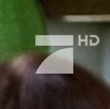
\includegraphics[width=3.5cm]{assets/images/logo_beispiel2.png} }}%
    \qquad
    \subfloat[]{{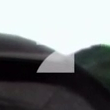
\includegraphics[width=3.5cm]{assets/images/logo_beispiel3.png} }}%
    \qquad
    \subfloat[]{{
\includegraphics[width=3.5cm]{assets/images/logo_beispiel4.png} }}%
    \qquad
    \subfloat[]{{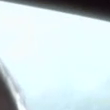
\includegraphics[width=3.5cm]{assets/images/logo_beispiel5.png} }}%
    \qquad
    \subfloat[]{{
\includegraphics[width=3.5cm]{assets/images/logo_beispiel6.png} }}%
    \caption{Logo mit verschiedenen Hintergründen}%
    \label{fig:logo2}%
\end{figure}
Eine grosse Schwierigkeit ist, dass bei manchen Hintergründen, vor allem bei weissen, das Logo abgeschnitten oder kaum bis gar nicht sichtbar ist.
Bei Abbildung~\ref{fig:logo2} (c) ist das Logo abgeschnitten, bei (d) ist es kaum sichtbar und bei (e) ist komplett verschwunden.
Das ist auch einfach zu erklären.
Wenn man für $a = 1$ (Weiss) in die Formel oben einsetzt erhält man: $f(1, b) = 1$, was bedeutet, dass das ganze Bild weiss ist und das Logo verschwunden ist.
Analog dazu, wenn man für $a = 0$ (Schwarz) einsetzt erhält man: $f(0, b) = b$, was bedeutet, dass das Logo, bei einem schwarzem Hintergrund, im ursprünglichen Zustand befindet.
Wegen dem kann man das Logo komplett herausfiltern und wieder verwenden wenn man das Logo mit einem schwarzen Hintergrund findet (siehe Abbildung~\ref{fig:logo2}f).

Ein andere Schwierigkeit ist, dass das Logo nicht unbedingt immer am gleichen Ort sein muss.
Zum Beispiel hat Prosieben 3 verschiedene Positionen (siehe Abbildung~\ref{fig:logo3}).
\begin{figure}[h]%
    \centering
    \subfloat[]{{
\includegraphics[width=6cm]{assets/images/logo_boarder_above.png} }}%
    \qquad
    \subfloat[]{{
\includegraphics[width=6cm]{assets/images/logo_boarder_side.png} }}%
    \qquad
    \subfloat[]{{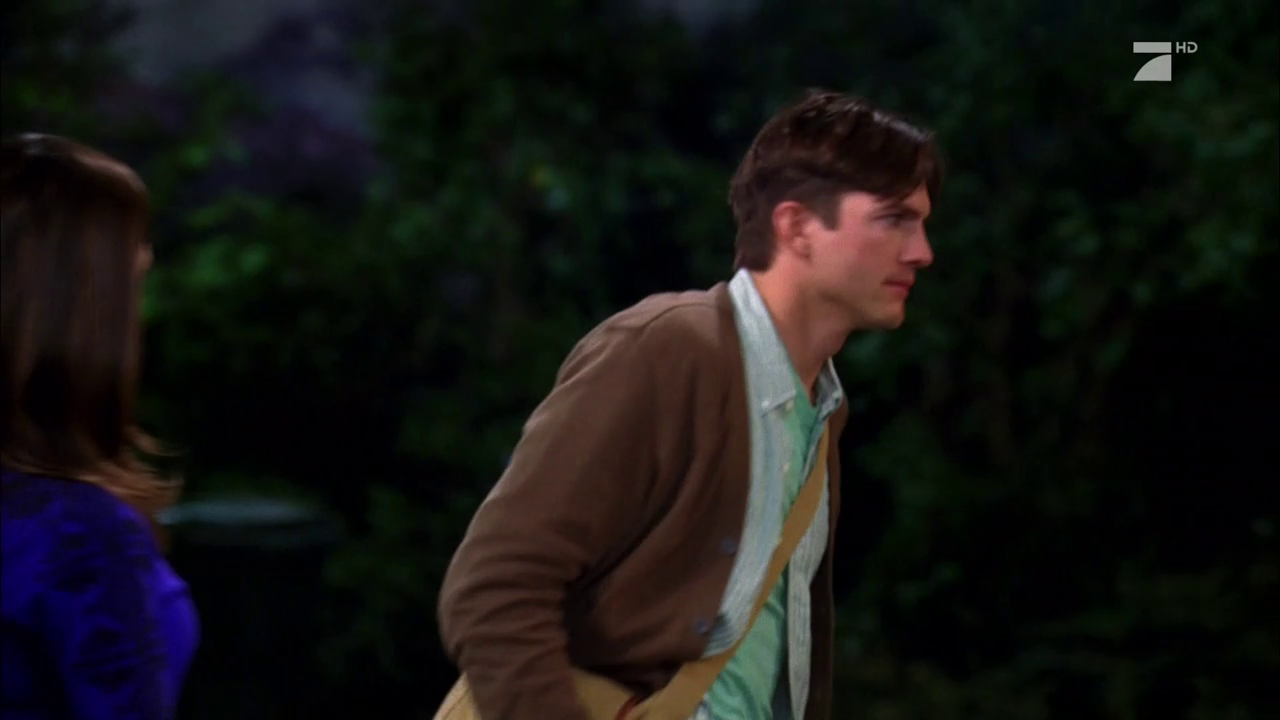
\includegraphics[width=6cm]{assets/images/logo_no_boarder.png} }}%
    \caption{Logo an verschiedenen Positionen}%
    \label{fig:logo3}%
\end{figure}

Alle diese Schwierigkeiten machen das erkennen eines Logo's ohne ein Neuronales Netzwerk extrem schwer.
Ein Neuronales Netzwerk hingegen löst das Probleme ziemlich elegant.

\section{Das Netzwerk trainieren}
\subsection{Farbe}
Die erste Frage, die sich stellt ist, ob man das Netzwerk mit farbigen oder mit schwarz-weiss Bildern trainieren will.
Dazu wird ein eigen gesammeltes Datensatz benutzt, das 7830 Prosieben Bilder besteht.
Aus dem wurde die Logos ausgeschnitten mit einem Rand von 10 Pixeln.



\chapter{Umsetzung}
\label{ch:umsetzung}

\chapter{Reflexion}
\label{ch:reflexion}

\clearpage
\phantomsection
\addcontentsline{toc}{chapter}{Literaturverzeichnis}
\nocite{*}
\bibliography{C:/Jetbrains/PyCharm/WerbeSkip/thoughts/arbeit/maturaarbeit}
\bibliographystyle{plain}

\clearpage
\phantomsection
\addcontentsline{toc}{chapter}{Abbildungsverzeichnis}

\listoffigures

\appendix


\chapter*{Ehrlichkeitserklärung}

Die eingereichte Arbeit ist das Resultat meiner persönlichen, selbstständigen Beschäftigung mit dem Thema.
Ich habe für sie keine anderen Quellen benutzt als die in den Verzeichnissen aufgeführten.
Sämtliche wörtlich übernommenen Texte (Sätze) sind als Zitate gekennzeichnet.

\vspace{2cm}
Insert Datum
\end{document}
